\documentclass[10pt]{exam}
\usepackage[hon]{template-for-exam}
\usepackage{enumitem}
\usepackage{tikz}
\usepackage{multicol,graphicx}
\usetikzlibrary{shadings,decorations.pathmorphing,arrows.meta}



\def\mytitle{Chapter 6 (Work \& Energy)}
\author{Rohrbach}
\date{\today}

\def\mymaketitle{
  \begin{flushleft}
    {\LARGE \textbf \mytitle \par}
  \end{flushleft}
}



\begin{document}


\mymaketitle



\newcommand{\stampbox}[1]{

  \hfill
  \begin{tikzpicture}[every text node part/.style={align=center}]
     \node[gray!50,draw,rounded corners] at (0,0) 
      {\sc Stamp \\ \sc Here \\ \small #1 \sc Points};
  \end{tikzpicture}
  \vspace{1em}
  
  \hrule

}

\begin{flushright}

  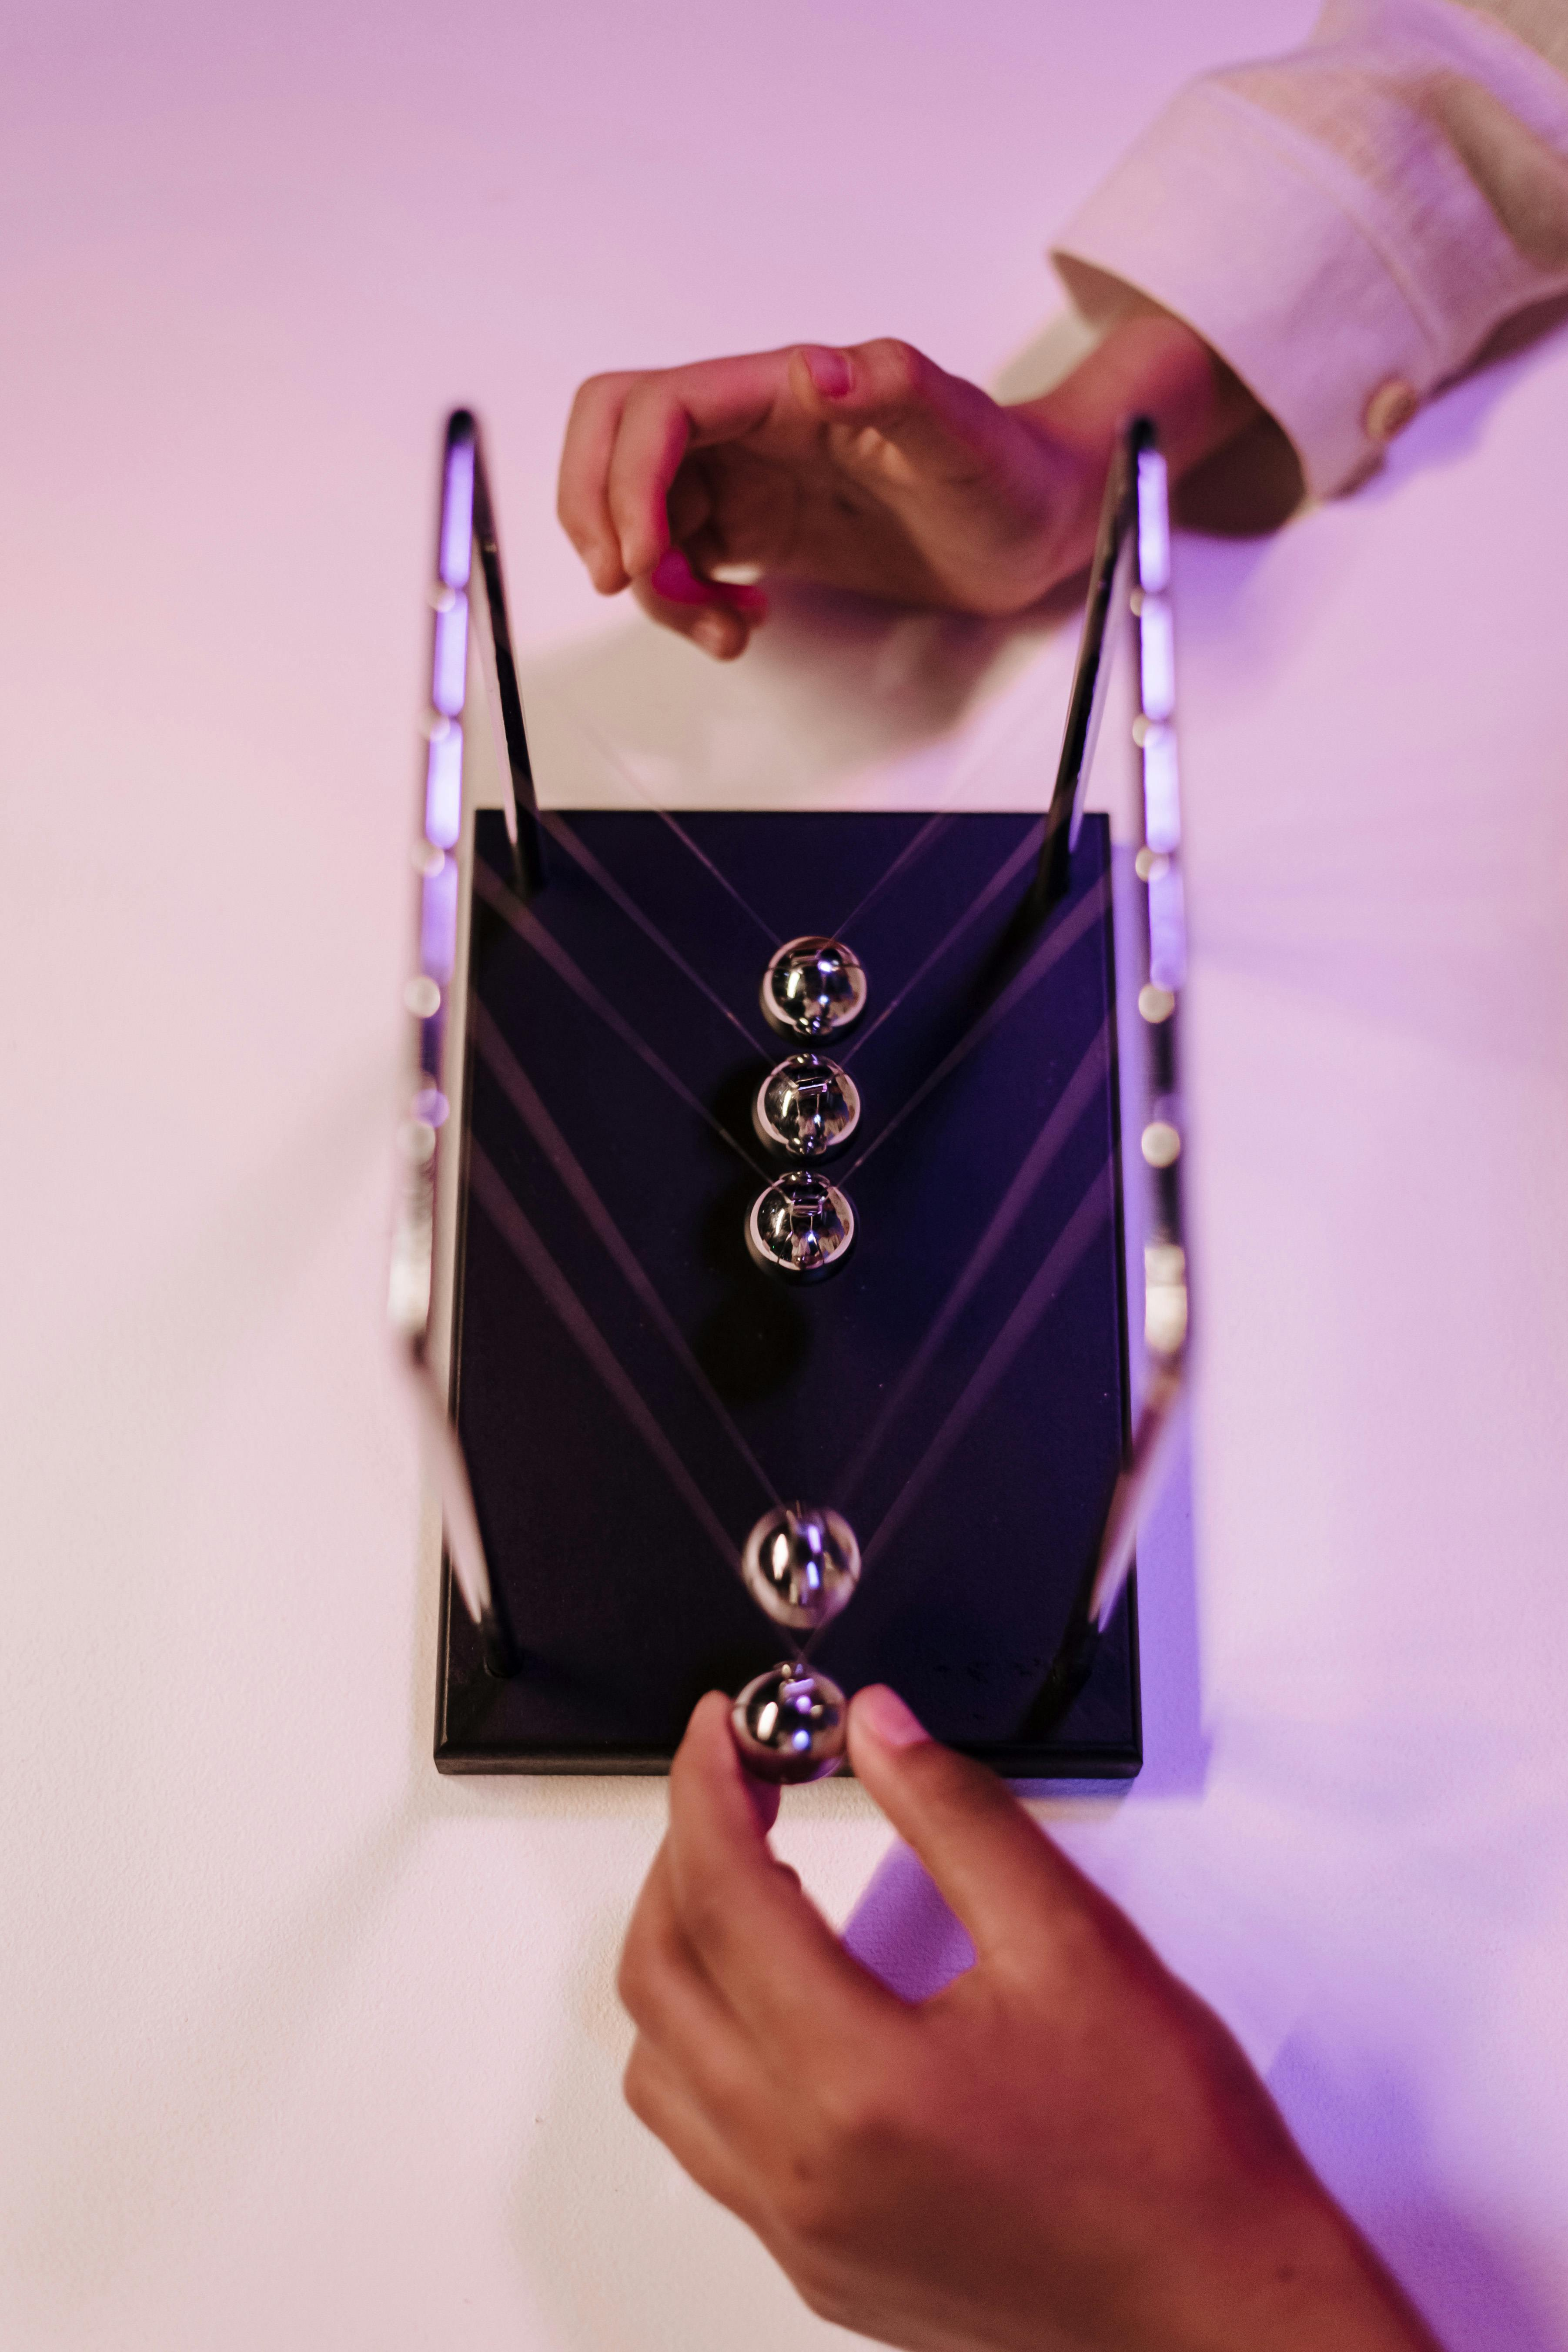
\includegraphics[height=4.5cm]{ncradle.jpg} \hspace{10em}
\end{flushright}

\section*{All Homework (collected Fri, Dec 13)}


%%%%%%%%%%%


\paragraph{Work, KE, PE} pp. 164-165 \#1, 3, 4, 15 ,16, 26, 27
\dotfill Complete by Fri, Dec 6

\stampbox{5}


%%%%%%%%%%%


\paragraph{Conservation of Energy} pp. 165-167 \#31, 32, 33, 37, 38, 47, 49
\dotfill Complete by Thu, Dec 12

\hfill \textbf{\emph{Homework Quiz}}

\stampbox{7}


%%%%%%%%%%%

\paragraph{Power} pp. 167 \#57, 60, 61
\dotfill Complete by Fri, Dec 13

\stampbox{3}


%%%%%%%%%%%

\paragraph{Bonus Problems!} \#5, 7, 41, 55
\dotfill Turn in separately.

\vspace{1em}
\hrule



\subsection*{Answers}

\begin{multicols}{3}

  \begin{itemize}[noitemsep]
    \item[1. ]  20,580 J
    \item[3. ] 2,322 J
    \item[4. ] (a) 1150 J;  (b) 6000 J
    \item[15.] 484 m/s
    \item[16.] (a) $\sqrt{3}$; \\ (b) 1/4
    \item[26.] 2,117 J
    \item[27.] 1.01 m
    \item[31.] 45.4 m/s
    \item[32.] 1.27 m
    \item[33.] 4.89 m/s
    %\item[34.] 6.44 m/s
    \item[37.] \SI{1.38e5}{\newton\per\meter}
    \item[38.] (a) 7.7 m/s; \\ (b) 25 cm
    %\item[40.] $v_2  = 25.0$ m/s;\\
    %           $v_3  = 10.8$ m/s;\\
    %           $v_4  = 18.8$ m/s
    \item[47.] $-332.5$ J
    \item[49.] (a) 15.3 m/s; \\ (b) $-1.03$ N
    \item[57.] 21.95 s
    \item[60.] 508.8 N 
    \item[61.] 2,686 N
  \end{itemize}
  
\end{multicols}

\section*{Equations}


\vspace{-1.5em}

\begin{align*}
  W    &= F_\parallel d &
  KE   &= \frac{1}{2} mv^2 &
  PE_g &= mgy &
  PE_e &= \frac{1}{2} kx^2
\end{align*}

\vspace{-1.5em}

\begin{align*}
  W &= \Delta KE &
  \Sigma E_0 + W_{NC} &= \Sigma E &
  P &= \frac{W}{t}
\end{align*}

\end{document}